\section{Base Decomposition: Why the Fit Fails}
\label{app:decomp}

Sweeping $K \in \{2,4,8,16,32,64\}$ at fixed output length fits
$T(K) = \kfitBase + \kfitSlope \cdot K$ with $R^2 = \kfitRsq$. The low $R^2$ is
itself informative: latency saturates above $K{=}16$, so the linear term is a
poor descriptions at the top of the range and the fit is carried by the bottom.
The intercept is therefore not interpretable as a floor.

\begin{figure}[h]
\centering
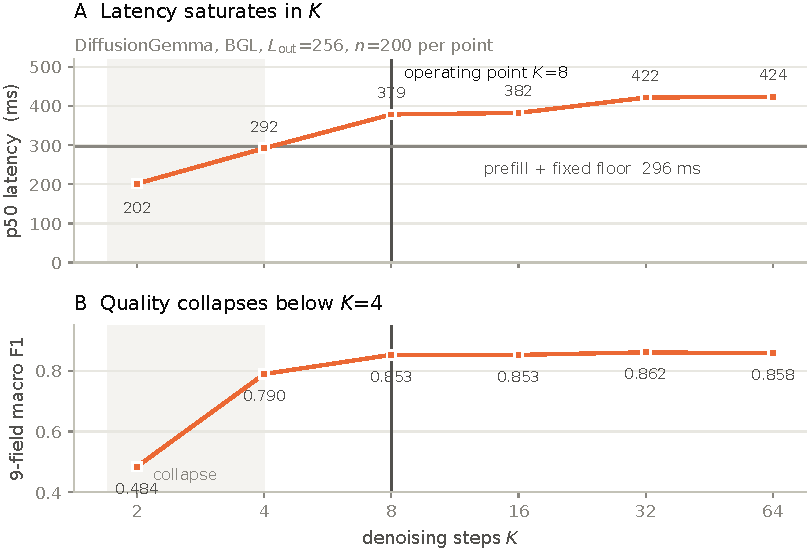
\includegraphics[width=0.85\linewidth]{figures/fig4_ksweep.pdf}
\caption{Denoising-step sweep. Latency saturates above $K{=}16$; quality is
flat above $K{=}8$. Halving $K$ from 8 to 4 saves $\sim$87\,ms because the
saving comes out of the small slice, while F1 falls from \kEightFone\ to
\kFourFone\ because the loss comes out of the whole.}
\label{fig:ksweep}
\end{figure}

Two measurement-based bounds do the work instead:

\begin{itemize}
\item \textbf{From $K{=}2$.} For any decomposition
$T(K) = \text{floor} + K \cdot c(K)$ with $c \geq 0$,
$\text{floor} \leq T(2) = 202$\,ms. At $K{=}8$ the denoising-attributable
share is $\geq 47\%$ of the \dgBase\,ms base.

\item \textbf{From the canvas step.} One additional canvas costs \dgStep\,ms
and is a $K{=}8$ denoising pass. So denoising is $\geq \dgStep / \dgBase = 32\%$
of the base. The first canvas's pass is somewhat cheaper than a marginal one,
but not by the $5\times$ the fitted intercept would require.
\end{itemize}

The honest range at $K{=}8$ is 32--47\% denoising against 53--68\% floor. The
exact split awaits profiler attribution.
